% Compile with pdfLaTeX: latexmk -pdf main.tex
\documentclass[t,aspectratio=169,11pt]{beamer}
% Beamer style rebuilt from the supplied lecture3.pdf reference.
% Standard TeX Live / Overleaf packages only. No system font paths.
\usepackage[T1]{fontenc}
\usepackage[utf8]{inputenc}
\usepackage{lmodern}
\usefonttheme[onlymath]{serif}
\usepackage{amsmath,amssymb,mathtools,bm}
\usepackage{booktabs,tabularx,array}
\usepackage{graphicx}
\usepackage{tikz,pgfplots}
\usepackage[most]{tcolorbox}
\usepackage{pgfpages}
\pgfplotsset{compat=1.18}
\usetikzlibrary{calc,arrows.meta,positioning}

\definecolor{titlered}{HTML}{D62B09}
\definecolor{bulletgreen}{HTML}{A8C99F}
\definecolor{definitionblue}{HTML}{E9F0F9}
\definecolor{takeawaypeach}{HTML}{FBECE6}
\definecolor{blueplot}{HTML}{4E79A7}
\definecolor{redplot}{HTML}{D95F59}
\definecolor{lightplot}{HTML}{8FB8DA}
\definecolor{inkplot}{HTML}{111111}
\setbeamercolor{normal text}{fg=black,bg=white}
\setbeamercolor{frametitle}{fg=titlered,bg=white}
\setbeamercolor{structure}{fg=titlered}
\setbeamercolor{itemize item}{fg=bulletgreen}
\setbeamercolor{itemize subitem}{fg=bulletgreen}
\setbeamercolor{footline}{fg=black,bg=white}
\setbeamercolor{block title}{fg=black,bg=definitionblue}
\setbeamercolor{block body}{fg=black,bg=definitionblue}
\setbeamersize{text margin left=0.75cm,text margin right=0.75cm}
\setbeamerfont{frametitle}{size=\fontsize{22}{25},series=\bfseries}
\setbeamerfont{footline}{size=\fontsize{5.5}{7}\selectfont}
\setbeamertemplate{navigation symbols}{}
\setbeamertemplate{itemize item}{\raise0.1ex\hbox{\small$\bullet$}}
\setbeamertemplate{itemize subitem}{\raise0.1ex\hbox{\scriptsize$\bullet$}}
\setbeamertemplate{frametitle}{%
  \vskip0.08cm
  \begin{beamercolorbox}[wd=\textwidth,center,sep=0pt]{frametitle}
    \usebeamerfont{frametitle}\strut\insertframetitle\strut\par
  \end{beamercolorbox}
  \vskip0.25cm
}
\setbeamertemplate{footline}{%
  \begin{beamercolorbox}[wd=\paperwidth,ht=0.25cm,dp=0.10cm,center]{footline}
    \usebeamerfont{footline}\insertframenumber
  \end{beamercolorbox}
}
\setlength{\parskip}{3pt}
\setlength{\abovedisplayskip}{6pt}
\setlength{\belowdisplayskip}{6pt}
\setlength{\abovedisplayshortskip}{4pt}
\setlength{\belowdisplayshortskip}{4pt}

\newcommand{\lead}[1]{{\small #1\par}\vspace{0.12cm}}
\newtcolorbox{definitionbox}{enhanced,colback=definitionblue,
  colframe=definitionblue,boxrule=0pt,arc=3pt,
  fontupper=\small,
  before upper={\setlength{\abovedisplayskip}{4pt}\setlength{\belowdisplayskip}{4pt}\setlength{\jot}{2pt}},
  left=6pt,right=6pt,top=4pt,bottom=4pt,
  before skip=4pt,after skip=5pt}
\newtcolorbox{takeaway}{enhanced,colback=takeawaypeach,
  colframe=takeawaypeach,boxrule=0pt,arc=3pt,
  fontupper=\small,left=6pt,right=6pt,top=4pt,bottom=4pt,
  before skip=6pt,after skip=0pt}
\newcommand{\demolink}[1]{\href{https://regression-lab-graduate-2026.whu38f.chatgpt.site/\##1}{\textcolor{titlered}{\textbf{Open web demo: #1}}}}
\newcommand{\R}{\mathbb{R}}
\newcommand{\E}{\mathbb{E}}
\DeclareMathOperator{\Var}{Var}
\DeclareMathOperator{\Cov}{Cov}
\DeclareMathOperator{\diag}{diag}
\DeclareMathOperator{\Col}{Col}
\DeclareMathOperator{\rank}{rank}
\DeclareMathOperator*{\argmin}{arg\,min}
\newcolumntype{Y}{>{\raggedright\arraybackslash}X}
\setbeameroption{hide notes}

%\newcommand{\sigm}{\operatorname{s}}
\newcommand{\sigm}{\sigma}
\newcommand{\logfigpath}{figures/}
\newcommand{\logfig}[1]{\input{\logfigpath#1.tex}}
\newcommand{\logprompt}[1]{\textcolor{titlered}{\textbf{#1}}}
\newcommand{\softplus}{\operatorname{softplus}}

\title{Logistic Regression: Likelihood, Optimization, and Softmax}
\author{Zihan Zhang}
\institute{COMP 5212: Machine Learning}
\date{}
\hypersetup{pdftitle={Logistic Regression: Likelihood, Optimization, and Softmax},pdfauthor={Zihan Zhang}}
\definecolor{slideorange}{HTML}{FF5500}
\definecolor{midgray}{HTML}{666666}
\newcommand{\SectionSlide}[2]{%
	\begin{frame}
		\centering
		\vfill
		{\color{slideorange}\fontsize{29}{34}\selectfont\bfseries #1\par}
		\vspace{0.38cm}
		{\color{midgray}\fontsize{16}{21}\selectfont #2\par}
		\vfill
	\end{frame}
}
% Uncomment for presenter notes on a second screen:
% \setbeameroption{show notes on second screen=right}
\begin{document}
	
	\begin{frame}
		\vspace{0.05cm}
		\hspace{-0.38cm}
\includegraphics[width=5.65cm]{../source/logo.png}
		\vspace{-0.15cm}
		\begin{center}
			{\fontsize{29}{35}\selectfont COMP 5212\par}
			\vspace{0.30cm}
			{\fontsize{32}{38}\selectfont Machine Learning\par}
			\vspace{0.35cm}
			{\fontsize{17}{21}\selectfont Instructor: Zihan Zhang\par}
			\vspace{0.25cm}
			{\fontsize{14}{18}\selectfont Lecture 5: Logistic Regression\par}
			\vspace{0.12cm}
			
		\end{center}
	\end{frame}
	

% Plan: learning goals / short list / static.
\begin{frame}[t]{Learning Goals}
\vspace{.03cm}
{\fontsize{13.2}{16.2}\selectfont
By the end of the lecture, you should be able to:
\begin{itemize}\setlength{\itemsep}{.18cm}
\item formulate logistic regression for binary outcomes;
\item derive least squares and logistic loss from likelihood;
\item derive and apply the gradient-descent update;
\item explain softmax regression and its categorical likelihood;
\item recognize softmax in classifiers, language models, and attention.
\end{itemize}}
\note{Use these goals as the map. Students already know least squares and basic matrix derivatives; connect each new expression to those earlier ideas. The final application distinguishes class probabilities from attention weights.}
\end{frame}

\section{Motivation}
% Plan: bridge from previous lecture / comparison / reveal probability.
\begin{frame}[t]{Same inputs, a different prediction}
\begin{columns}[T,onlytextwidth]
\begin{column}{.47\textwidth}
\begin{definitionbox}
\textbf{Linear regression}\par
Sensor readings $x$\par\vspace{3pt}
$\longrightarrow$ electricity consumption $Y\in\R$
\[\widehat y=b+w^{\mathsf T}x.\]
\end{definitionbox}
\end{column}
\begin{column}{.47\textwidth}
\begin{definitionbox}
\textbf{Binary classification}\par
Sensor readings $x$\par\vspace{3pt}
$\longrightarrow$ defective or acceptable $Y\in\{0,1\}$
\uncover<2->{\[\pi(x)=\Pr(Y=1\mid x).\]}
\end{definitionbox}
\end{column}
\end{columns}
\vspace{.3cm}
\logprompt{What should replace a real-valued prediction?}
\uncover<2->{\begin{takeaway}Predict a probability first; use it to make a decision.\end{takeaway}}
\note{Pause before revealing the right-hand probability. Reuse the manufacturing setting from the linear-regression lecture: the inputs can be similar even though the output is now an event. This changes the conditional response model and the fitting criterion.}
\end{frame}
% Plan: application / figure or comparison / staged reveal.
\begin{frame}[t]{Motivation: detecting defective parts}
\lead{A sensor measures process intensity. Inspection records whether each part is defective}
\begin{columns}[T,onlytextwidth]
\begin{column}{.59\textwidth}\logfig{motivation}\end{column}
\begin{column}{.38\textwidth}\small
$x$: sensor measurement\par
$y=1$: defective\par
$y=0$: acceptable
\vspace{.25cm}\par
\logprompt{What should we predict for the next part?}
\uncover<2->{\vspace{.15cm}\par
\[\Pr(Y=1\mid x).\]
A probability expresses uncertainty.}
\end{column}
\end{columns}
\note{Ask students whether the next part must have the same label as its nearest neighbor. The overlap motivates a probability rather than a deterministic physical rule. The sensor is only one available feature; temperature, vibration and machine age could also be included. This is a realistic application setting, but the observations are deliberately constructed, not an industrial dataset. Do not imply the association is causal.}
\end{frame}

% Plan: application / figure or comparison / staged reveal.
\begin{frame}[t]{Probabilities and decisions}
\small\renewcommand{\arraystretch}{1.6}
\begin{tabularx}{\textwidth}{@{}cYY@{}}
\toprule
\textbf{Part}&\textbf{Predicted defect probability}&\textbf{Decision at threshold $0.5$}\\\midrule
A&$0.55$&Flag\\
B&$0.95$&Flag\\\bottomrule
\end{tabularx}\par
\vspace{.35cm}
\logprompt{Do these predictions carry the same information?}
\uncover<2->{\vspace{.2cm}\par\small
\begin{itemize}\setlength{\itemsep}{.2cm}
\item Probabilities help rank inspection priorities.
\item A decision also depends on the cost of each mistake.
\end{itemize}}
\vfill
\begin{takeaway}First estimate a probability. Then choose the action appropriate to the application.\end{takeaway}
\note{The two probabilities are hypothetical. A binary flag discards the difference between 55 percent and 95 percent risk. Ask which part should be inspected first when only one inspection slot is available and costs are otherwise equal. The decision threshold can be selected according to the application; this lecture focuses on fitting the probabilities. A numerical probability is useful only to the extent that it agrees with the data-generating distribution; logistic form alone does not guarantee calibration.}
\end{frame}

% Plan: application / figure or comparison / staged reveal.
\begin{frame}[t]{OLS with binary responses}
\begin{columns}[T,onlytextwidth]
\begin{column}{.59\textwidth}\logfig{ols-binary}\end{column}
\begin{column}{.38\textwidth}\small
For $Y\in\{0,1\}$,
\[\E[Y\mid x]=\Pr(Y=1\mid x).\]
\vspace{.12cm}\par
An unconstrained line can predict below $0$ or above $1$.
\uncover<2->{\vspace{.2cm}\par
\logprompt{How can a linear score become a valid probability?}}
\end{column}
\end{columns}
\vfill
\begin{takeaway}OLS can fit binary labels. Its unrestricted linear predictions need not respect probability bounds.\end{takeaway}
\note{Avoid claiming that least squares cannot be applied to binary outcomes or that it requires Gaussian responses simply to define an estimator. The issue shown here is the unrestricted linear probability model: its predictions can leave the unit interval, and the Bernoulli conditional variance changes with the mean. Squared probability error is itself a valid proper scoring rule; the Bernoulli likelihood motivates the cross-entropy used in this lecture. The OLS line is computed from the same constructed data as the motivation plot.}
\end{frame}

\SectionSlide{Forumulation}{}
\section{Problem formulation}

% Plan: binary model / equation or figure / reveal where marked.
\begin{frame}[t]{The logistic function}
\begin{columns}[T,onlytextwidth]
\begin{column}{.59\textwidth}\logfig{sigmoid}\end{column}
\begin{column}{.38\textwidth}\small
\[\sigm(z)=\frac{1}{1+e^{-z}}.\]
\vspace{.15cm}\par
\begin{itemize}\setlength{\itemsep}{.18cm}
\item $\sigm(0)=1/2$.
\item $0<\sigm(z)<1$ for finite $z$.
\item $\sigm(-z)=1-\sigm(z)$.
\end{itemize}
\uncover<2->{\[\sigm'(z)=\sigm(z)(1-\sigm(z)).\]}
\end{column}
\end{columns}
\vfill
\begin{takeaway}The score is unbounded. The probability stays between zero and one.\end{takeaway}
\note{Ask students to identify the score for probability one half and the scores needed for probabilities near zero or one. Derive the derivative by differentiating (1+exp(-z)) inverse. Its maximum is one quarter at zero, and it becomes small in either tail. This saturation will matter for curvature in gradient-based optimization. The logistic function is a modeling choice, not the only possible link for binary probabilities.}
\end{frame}

% Plan: binary model / equation or figure / reveal where marked.
\begin{frame}[t]{A linear model for log-odds}
\lead{For $0<\pi(x)<1$, odds are $\pi(x)/(1-\pi(x))$}
\begin{definitionbox}
\[
\begin{aligned}
\log\frac{\pi(x)}{1-\pi(x)}&=b+w^{\mathsf T}x=z,\\[6pt]
\frac{\pi(x)}{1-\pi(x)}&=e^z,\\[6pt]
\pi(x)&=\frac{e^z}{1+e^z}=\boxed{\sigm(b+w^{\mathsf T}x)}.
\end{aligned}
\]
\end{definitionbox}
\uncover<2->{\begin{takeaway}Logistic regression assumes that log-odds are linear in the chosen features.\end{takeaway}}
\note{The transformation turns a probability in (0,1) into any real number, making an additive linear model possible. Stress that this is an assumption about conditional log-odds, not a theorem that every binary dataset must satisfy. Local linear approximation to a smooth log-odds function is one motivation for a useful baseline. Feature expansion can make the log-odds nonlinear in the original measurements while preserving linearity in the fitted coefficients.}
\end{frame}


% Plan: precise formulation / equations and examples / progressive when marked.
\begin{frame}[t]{Decision thresholds and boundaries}
\begin{columns}[T,onlytextwidth]
\begin{column}{.59\textwidth}\logfig{boundary}\end{column}
\begin{column}{.38\textwidth}\small
For $0<\tau<1$, predict class $1$ if $\pi(x)\ge\tau$.
\[
b+w^{\mathsf T}x\ge\log\frac{\tau}{1-\tau}.
\]
\vspace{.1cm}\par
$\tau=0.5$: score boundary $0$.\par
$\tau=0.8$: score boundary $\log 4$.
\end{column}
\end{columns}
\vfill
\begin{takeaway}Changing the threshold moves the decision boundary without refitting the probability model.\end{takeaway}
\note{The figure uses score -1+x1+0.8x2, with constructed class labels. Since the logistic function is strictly increasing, taking the logit of the threshold yields the displayed inequality. For fixed linear features and nonzero w, the boundary is a hyperplane. Raising the threshold shrinks the region classified as positive. This plot illustrates fixed-model decisions, not estimates fitted to the shown points.}
\end{frame}

% Plan: precise formulation / equations and examples / progressive when marked.
\begin{frame}[t]{Worked example: score to decision}
\lead{$z=-2+0.8x$, $\pi=\sigm(z)$, decision threshold $\tau=0.7$}
\small\renewcommand{\arraystretch}{1.7}
\begin{tabular*}{\textwidth}{@{\extracolsep{\fill}}cccc@{}}
\toprule $x$&\textbf{Score $z$}&\textbf{Probability $\pi$}&\textbf{Predicted class}\\\midrule
$2$&\uncover<2->{$-0.4$}&\uncover<2->{$0.401$}&\uncover<2->{$0$}\\
$4$&\uncover<2->{$1.2$}&\uncover<2->{$0.769$}&\uncover<2->{$1$}\\\bottomrule
\end{tabular*}\par
\vspace{.35cm}
\logprompt{At what sensor value does the decision change?}
\uncover<3->{\[
x=\frac{2+\log(0.7/0.3)}{0.8}\approx3.559.
\]}
\note{Give students 20 seconds for the table, then reveal it. Pause again before the threshold calculation. Distinguish the raw measurement x, the real-valued score z, the probability pi and the binary decision. The threshold is an application choice separate from the model parameters. At exactly the boundary, the chosen greater-than-or-equal convention predicts class one.}
\end{frame}

% Plan: parameter-fitting problem / model definition / reveal loss question.
\begin{frame}[t]{What do we learn from the data?}
\begin{definitionbox}
\[
\mathcal D=\{(x_i,y_i)\}_{i=1}^n,\qquad y_i\in\{0,1\},
\qquad \pi_i(\theta)=\sigm(\widetilde x_i^{\mathsf T}\theta).
\]
\[
\widehat\theta=\argmin_{\theta\in\R^p}J(\theta).
\]
\end{definitionbox}
\vspace{.2cm}
\logprompt{Which objective rewards good probability predictions?}
\uncover<2->{\par\vspace{.15cm}\small
Compare the probability assigned to each observed label.
\begin{takeaway}Maximum likelihood turns this requirement into a loss function.\end{takeaway}}
\note{The probability model has been specified; the fitting criterion is still to be derived. Accuracy alone treats probability .51 and .99 the same for a positive label. Likelihood provides a differentiable probability-based criterion. An argmin is a useful formulation here, but the separation caveat later explains when no finite unregularized optimizer exists.}
\end{frame}

\SectionSlide{MLE Interpretation}{}
% Maximum-likelihood module. Uses the shared theme and logistic-macros.tex.
% Notation: X has rows x-tilde_i^T; theta includes the intercept.
\section{Maximum likelihood: from least squares to cross-entropy}

% MLE 01. Point: likelihood varies parameters while the observed sample stays fixed.
% Layout: one conditional-likelihood display, followed by a staged factorization.
% Reveal: 2 adds conditional independence; 3 states the estimation principle.
\begin{frame}[t]{What does conditional likelihood measure?}
\small
We observe the inputs $X$ and responses $y$. A model assigns them
\[
\mathcal L(\theta;y\mid X)=f_\theta(y\mid X).
\]
As a likelihood, this is a function of $\theta$, with $X$ and $y$ held fixed.

\uncover<2->{
\vspace{.15cm}
If the responses are independent conditional on $X$,
\[
f_\theta(y\mid X)=\prod_{i=1}^n
f_\theta(y_i\mid\widetilde x_i).
\]}
\uncover<3->{
\begin{takeaway}
Maximum likelihood chooses parameters that give the observed responses the
largest joint probability mass or density, within the chosen model.
\end{takeaway}}
\note{The same expression has two roles. As a sampling model, theta is fixed and y varies; as a likelihood, the observed y is fixed and theta varies. We condition on the inputs, so we do not need a probability model for X to define this criterion. The displayed factorization assumes conditionally independent responses and that each response distribution depends on X through its own feature vector. For a continuous response, f is a density, not the probability of observing an exact real number. A likelihood is also not a probability distribution over theta. We first revisit Gaussian linear regression, then return to the binary response model.}
\end{frame}

% MLE 02. Point: the Gaussian error assumption turns a residual into a density.
% Layout: analytic residual-density plot beside the conditional model.
% Reveal: 2 connects increasing absolute residual to decreasing density.
\begin{frame}[t]{Gaussian errors assign density to residuals}
\small
For this comparison, first let the response be real-valued: $y_i\in\R$.
\begin{columns}[T,onlytextwidth]
\begin{column}{.56\textwidth}
\logfig{mle-gaussian-residual}
\end{column}
\begin{column}{.41\textwidth}
\[
Y_i=\widetilde x_i^{\mathsf T}\theta+\varepsilon_i,
\]
\[
\varepsilon_i\mid X\overset{\mathrm{iid}}{\sim}
\mathcal N(0,\sigma^2),\qquad\sigma>0.
\]
For the observed response, the residual is
\[
r_i(\theta)=y_i-\widetilde x_i^{\mathsf T}\theta.
\]
\uncover<2->{
At fixed $\sigma$, a larger $|r_i|$ receives a smaller Gaussian density.}
\end{column}
\end{columns}
\note{We temporarily change the response family to revisit linear regression; this slide is not a Gaussian model for a binary variable. Conditional on the design, the errors are independent and identically distributed with mean zero and the same positive variance. Consequently the responses are independent but generally have different conditional means. The plotted curve is the analytic standard normal density, so sigma equals one in the illustration. The marked residuals zero and two have densities about 0.399 and 0.054. These are density heights, not point probabilities; the area over an interval gives a probability. The Gaussian assumption is what connects this particular likelihood calculation to squared residuals.}
\end{frame}

% MLE 03. Point: the Gaussian negative log-likelihood differs from SSE only by fixed terms and scale.
% Layout: product likelihood, negative logarithm, then the coefficient optimization.
% Reveal: 2 takes the logarithm; 3 discards theta-independent terms for fixed sigma.
\begin{frame}[t]{The Gaussian likelihood leads to squared error}
\small
\[
\mathcal L(\theta,\sigma;y\mid X)
=\prod_{i=1}^n\frac{1}{\sqrt{2\pi\sigma^2}}
\exp\!\left[-\frac{(y_i-\widetilde x_i^{\mathsf T}\theta)^2}{2\sigma^2}\right].
\]
\uncover<2->{
\[
-\log\mathcal L
=\underbrace{\frac n2\log(2\pi\sigma^2)}_{\text{constant in }\theta}
+\frac{1}{2\sigma^2}\underbrace{\sum_{i=1}^n
(y_i-\widetilde x_i^{\mathsf T}\theta)^2}_{\operatorname{Square Error}(\theta)}.
\]}
\uncover<3->{
\begin{takeaway}
For any fixed $\sigma>0$, maximizing this likelihood over $\theta$ is equivalent to
\[
\min_\theta\operatorname{Square Error}(\theta)
=\min_\theta\lVert y-X\theta\rVert_2^2.
\]
\end{takeaway}}
\note{Take the negative logarithm one factor at a time. The exponential contributes the squared residual divided by twice the variance, and the normalizing factors contribute n/2 times log(2 pi sigma squared). At any fixed positive sigma, the first term is constant in theta and the second has a positive scale, so the minimizers are exactly the least-squares solutions. If sigma is also estimated and the minimum SSE is positive, the joint Gaussian MLE has a least-squares coefficient vector and variance SSE/n. If the data can be fit exactly, the likelihood becomes unbounded as sigma approaches zero, so a joint finite MLE with strictly positive variance need not exist. We keep sigma fixed here to isolate the coefficient argument.}
\end{frame}



% MLE 05. Point: full rank determines unique coefficients; rank deficiency leaves a family.
% Layout: full-rank result above a staged rank-deficient alternative.
% Reveal: 2 adds the pseudoinverse family and the minimum-norm selection.


% MLE 06. Point: a Bernoulli model rewards probability assigned to the realized label.
% Layout: binary conditional model followed by a two-case probability expression.
% Reveal: 2 writes both cases in one algebraic formula.
\begin{frame}[t]{The probability of an observed binary label}
\small
Now $y_i\in\{0,1\}$ and
\[
Y_i\mid\widetilde x_i;\theta\sim\operatorname{Bernoulli}(\pi_i),
\qquad \pi_i=\sigm(\widetilde x_i^{\mathsf T}\theta).
\]
The model assigns the observed label probability
\[
\Pr(Y_i=y_i\mid\widetilde x_i;\theta)
=\begin{cases}
\pi_i,&y_i=1,\\[4pt]
1-\pi_i,&y_i=0.
\end{cases}
\]
\uncover<2->{
\begin{definitionbox}
\[
\Pr(Y_i=y_i\mid\widetilde x_i;\theta)
=\boxed{\pi_i^{y_i}(1-\pi_i)^{1-y_i}}.
\]
\end{definitionbox}}
\note{We now return to the binary labels and logistic mean model introduced earlier. Ask the audience to check the exponents separately for y equal to zero and one. Pi is always the probability of class one; it is not always the probability of the label we actually observed. A negative label receives probability one minus pi. The Bernoulli model specifies conditional variance pi times one minus pi, so there is no separate constant residual variance parameter analogous to sigma squared. The logistic link was already chosen as a model for the mean; the Bernoulli likelihood by itself does not determine that link.}
\end{frame}

% MLE 07. Point: conditional Bernoulli likelihood becomes average binary cross-entropy.
% Layout: product, log, and mean negative log-likelihood in separate display bands.
% Reveal: 2 takes the log; 3 changes sign and divides by n.
\begin{frame}[t]{Bernoulli likelihood and binary cross-entropy}
\small
Conditional independence gives
\[
\mathcal L(\theta;y\mid X)
=\prod_{i=1}^n\pi_i^{y_i}(1-\pi_i)^{1-y_i}.
\]
\uncover<2->{
\[
\log\mathcal L(\theta)
=\sum_{i=1}^n\left[y_i\log\pi_i+(1-y_i)\log(1-\pi_i)\right].
\]}
\uncover<3->{
\begin{definitionbox}
\[
J(\theta)=-\frac1n\log\mathcal L(\theta)
=\frac1n\sum_{i=1}^n
\underbrace{\left[-y_i\log\pi_i-(1-y_i)\log(1-\pi_i)\right]}_{\text{binary cross-entropy }\ell_i(\theta)}.
\]
\end{definitionbox}
Natural logarithms are used throughout. Averaging preserves any unpenalized optimum.}
\note{Independence is the step that makes the joint probability a product. Because log is strictly increasing, maximizing the product and maximizing its log have the same optimizers when they exist. Negating converts a maximization into a minimization; dividing by n yields the mean loss used in the optimization section. The division changes gradient scale and must be coordinated with a penalty coefficient when a regularizer is added. Products of many probabilities may underflow numerically, another reason to work with log-likelihoods. Calling this maximum likelihood does not guarantee a finite maximizer: separation can send coefficient magnitudes to infinity. That existence issue is examined later.}
\end{frame}

% MLE 08. Point: substituting the logistic link gives softplus minus the observed-label score.
% Layout: two log identities, one substitution, then the boxed score-space loss.
% Reveal: 2 substitutes into BCE; 3 cancels the two softplus coefficients.
\begin{frame}[t]{Express the same loss through the score}
\small
For $z_i=\widetilde x_i^{\mathsf T}\theta$, define
$\softplus(z)=\log(1+e^z)$. Then
\[
\log\pi_i=z_i-\softplus(z_i),
\qquad
\log(1-\pi_i)=-\softplus(z_i).
\]
\uncover<2->{
\[
\ell_i(\theta)
=-y_i\bigl[z_i-\softplus(z_i)\bigr]
+(1-y_i)\softplus(z_i).
\]}
\uncover<3->{
\begin{definitionbox}
\[
\boxed{\ell_i(\theta)=\softplus(z_i)-y_i z_i},
\qquad
J(\theta)=\frac1n\sum_{i=1}^n\ell_i(\theta).
\]
\end{definitionbox}
This is binary cross-entropy expressed through the logistic score.}
\note{Use pi equal to exp(z) divided by one plus exp(z), and one minus pi equal to one divided by one plus exp(z), to obtain the two log identities. After substitution, the coefficients multiplying softplus are y and one minus y, so they add to one. This form will make the derivative particularly simple in the next module. It is exactly the earlier Bernoulli loss composed with the logistic link, not a different statistical criterion. The literal evaluation log(1+exp(z)) can overflow. A stable implementation uses max(z,0)-y z+log1p(exp(-abs(z))) or a library binary-cross-entropy-with-logits routine. The displayed formula is for the mathematical derivation.}
\end{frame}

% MLE 09. Point: pi is class-one probability; likelihood uses each observed label's probability.
% Layout: three-observation table, then joint likelihood and average loss.
% Reveal: 2 fills the observed-label probabilities; 3 computes product and mean NLL.
\begin{frame}[t]{Which probabilities enter the likelihood?}
\small
Illustrative predictions for three conditionally independent observations:\par
\vspace{.08cm}
\renewcommand{\arraystretch}{1.5}
\begin{tabular*}{\textwidth}{@{\extracolsep{\fill}}cccl@{}}
\toprule
$i$&$y_i$&$\pi_i$&\textbf{Observed-label probability}\\
\midrule
$1$&$1$&$0.8$&\uncover<2->{$0.8$}\\
$2$&$0$&$0.7$&\uncover<2->{$1-0.7=0.3$}\\
$3$&$1$&$0.4$&\uncover<2->{$0.4$}\\
\bottomrule
\end{tabular*}
\uncover<3->{
\[
\mathcal L=0.8\times0.3\times0.4=0.096,
\qquad J=-\frac13\log(0.096)\approx0.781.
\]
The second observation contributes $-\log(0.3)$, because its label is $0$.}
\note{These probabilities are constructed for arithmetic practice, not estimated from an empirical dataset. Before revealing the last column, ask which factor should be used for the second observation. The correct factor is 0.3, not 0.7. The individual negative log-likelihoods are approximately 0.2231, 1.2040, and 0.9163, which sum to 2.3434 and average to 0.7811. No thresholded prediction enters this calculation. A probability of 0.4 for a positive label contributes a finite loss even if a threshold of one half would classify it incorrectly. Changing the decision threshold cannot change this likelihood when the fitted probabilities are held fixed.}
\end{frame}

% MLE 10. Point: the response family and mean model determine the likelihood-based loss.
% Layout: compact Gaussian/Bernoulli comparison, followed by two modeling caveats.
% Reveal: 2 distinguishes the fitting principle from the link choice and from the definition of OLS.
\begin{frame}[t]{Response models and their fitting losses}
\small
\renewcommand{\arraystretch}{1.45}
\begin{tabularx}{\textwidth}{@{}lYY@{}}
\toprule
&\textbf{Gaussian linear regression}&\textbf{Logistic regression}\\
\midrule
Response family&Gaussian on $\R$&Bernoulli on $\{0,1\}$\\
Conditional mean&$\widetilde x_i^{\mathsf T}\theta$&$\sigm(\widetilde x_i^{\mathsf T}\theta)$\\
Conditional variance&$\sigma^2$&$\pi_i(1-\pi_i)$\\
Fitting loss&Squared error&Binary cross-entropy\\
\bottomrule
\end{tabularx}
\uncover<2->{
\vspace{.2cm}
\begin{itemize}\setlength{\itemsep}{.12cm}
\item A Bernoulli likelihood still needs a mean model. MLE does not force the logistic link.
\item OLS is defined by minimizing squared error. Gaussian errors give it one likelihood interpretation.
\end{itemize}}
\note{The loss row suppresses positive scale factors and parameter-independent terms from the fixed-variance Gaussian negative log-likelihood. The two choices in a conditional regression model are a response family and a model for its mean. A Bernoulli family combined with a probit mean, for example, is also fit by maximum likelihood but is not logistic regression. Conversely, least squares is an optimization criterion that remains defined without Gaussian noise, including when applied to binary observations. Its statistical properties then depend on the assumptions appropriate to that setting. The Gaussian assumptions in this module explain a likelihood interpretation of least squares; they are not prerequisites for writing or solving the OLS problem. Next we differentiate the logistic objective and examine how to optimize it.}
\end{frame}

\SectionSlide{Optimization}{}
\section{Optimization with gradient descent}
% Plan: interpret per-observation loss / probability-loss curves / static.
\begin{frame}[t]{A confident mistake incurs a large loss}
\begin{columns}[T,onlytextwidth]
\begin{column}{.60\textwidth}\logfig{logloss}\end{column}
\begin{column}{.36\textwidth}\small
\[
\ell(y,\pi)=\begin{cases}
-\log\pi,&y=1,\\[3pt]
-\log(1-\pi),&y=0.
\end{cases}
\]
For an observed positive label:
\[
\pi=0.9\Rightarrow\ell\approx0.105,
\]
\[
\pi=0.01\Rightarrow\ell\approx4.605.
\]
\end{column}
\end{columns}
\begin{takeaway}The loss uses probability confidence, not just the predicted class.\end{takeaway}
\note{This is loss as a function of a single predicted probability. It is different from the later optimization curve, which shows average loss against iteration. For a positive label the loss diverges as its assigned probability approaches zero; the negative-label curve is reflected horizontally. The curves are analytical and the numerical examples use natural logs.}
\end{frame}

% Plan: derive the score derivative / progressive derivation / reveal cancellation.
\begin{frame}[t]{The derivative becomes a prediction residual}
\lead{For one observation: $\ell=-y\log\pi-(1-y)\log(1-\pi)$ and $\pi=\sigm(z)$}
\begin{definitionbox}
\[
\frac{\partial\ell}{\partial\pi}=-\frac{y}{\pi}+\frac{1-y}{1-\pi},
\qquad \frac{\partial\pi}{\partial z}=\pi(1-\pi).
\]
\uncover<2->{\[
\frac{\partial\ell}{\partial z}
=\left(-\frac{y}{\pi}+\frac{1-y}{1-\pi}\right)\pi(1-\pi)
=\boxed{\pi-y}.
\]}
\end{definitionbox}
\uncover<2->{\begin{takeaway}The model probability minus the observed label drives the update.\end{takeaway}}
\note{Pause before multiplying the two derivatives. The sigmoid derivative cancels the denominators introduced by the Bernoulli log loss. For a positive example with low probability, pi minus y is negative, so descent tends to increase its score. Do not add another sigmoid-derivative factor after this cancellation. All expressions are for finite scores.}
\end{frame}

% Plan: assemble gradients / matrix equations / reveal link to OLS.
\begin{frame}[t]{From one observation to the whole sample}
\begin{definitionbox}
\[
\nabla_\theta\ell_i=(\pi_i-y_i)\widetilde x_i,
\qquad J(\theta)=\frac1n\sum_{i=1}^n\ell_i.
\]
\[
\boxed{\nabla J(\theta)=\frac1nX^{\mathsf T}(\pi-y)},
\qquad \pi=\sigm(X\theta).
\]
\end{definitionbox}
\uncover<2->{\small
\begin{tabularx}{\textwidth}{@{}lYY@{}}\toprule
&\textbf{Prediction}&\textbf{Gradient of mean loss}\\\midrule
Least squares&$X\theta$&$X^{\mathsf T}(X\theta-y)/n$\\
Logistic regression&$\sigm(X\theta)$&$X^{\mathsf T}(\pi-y)/n$\\\bottomrule
\end{tabularx}}
\note{Least squares in this table uses SSE divided by 2n; logistic regression uses mean binary cross-entropy without a factor of one half. The algebraic pattern is the same, but the predictions and curvature differ. The intercept is already represented by the first column of X.}
\end{frame}

% Plan: curvature and convexity / two equations / reveal implication.
\begin{frame}[t]{The logistic objective is convex}
\begin{definitionbox}
\[
\nabla^2J(\theta)=\frac1nX^{\mathsf T}D(\theta)X,
\quad D(\theta)=\diag\!\bigl(\pi_i(1-\pi_i)\bigr).
\]
\[
v^{\mathsf T}\nabla^2J(\theta)v
=\frac1n\sum_i\pi_i(1-\pi_i)(\widetilde x_i^{\mathsf T}v)^2\ge0.
\]
\end{definitionbox}
\uncover<2->{\small
\begin{itemize}\setlength{\itemsep}{.15cm}
\item Every finite stationary point is a global minimum.
\item Full column rank gives positive curvature at finite $\theta$.
\end{itemize}
\begin{takeaway}Convexity does not by itself guarantee that a finite minimizer exists.\end{takeaway}}
\note{D has strictly positive diagonal entries at finite scores, so a full-column-rank X gives a positive-definite Hessian there. Curvature can nevertheless approach zero as scores diverge. Later the two-point separation example shows a strictly convex objective with an unattained infimum. Feature scaling and near-collinearity still influence optimization.}
\end{frame}

% Plan: algorithm / numbered procedure / static.
\begin{frame}[t]{Gradient descent for logistic regression}
\lead{No general OLS-style closed form. Initialize $\theta^{(0)}=0$; choose $\eta>0$}
\begin{definitionbox}
\[
\begin{aligned}
z^{(t)}&=X\theta^{(t)},\\[3pt]
\pi^{(t)}&=\sigm\!\left(z^{(t)}\right),\\[3pt]
g^{(t)}&=\frac1nX^{\mathsf T}(\pi^{(t)}-y),\\[3pt]
\theta^{(t+1)}&=\theta^{(t)}-\eta g^{(t)}.
\end{aligned}
\]
\end{definitionbox}
\small Monitor the objective and $\|g^{(t)}\|_2$; use a maximum iteration count.
\note{This is full-batch gradient descent. Each update costs O(np) and does not require a matrix inverse. At zero initialization all binary probabilities equal one half. For large datasets one can replace the full gradient by a mini-batch average, producing stochastic rather than necessarily monotone loss traces. Fit any feature scaling on training data only.}
\end{frame}

% Plan: arithmetic example / table and reveal / two stages.
\begin{frame}[t]{One gradient step by hand}
\lead{A separate three-observation example: $\theta^{(0)}=(b,w)=(0,0)$ and $\eta=1$}
\begin{columns}[T,onlytextwidth]
\begin{column}{.34\textwidth}
\small\renewcommand{\arraystretch}{1.5}
\begin{tabular}{@{}rrr@{}}\toprule
$x_i$&$y_i$&$\pi_i^{(0)}$\\\midrule
$-1$&$0$&$1/2$\\
$0$&$0$&$1/2$\\
$1$&$1$&$1/2$\\\bottomrule
\end{tabular}
\end{column}
\begin{column}{.61\textwidth}
\logprompt{Compute the average residual and its feature-weighted average.}
\uncover<2->{\[
g^{(0)}=\begin{bmatrix}1/6\\-1/3\end{bmatrix},
\qquad\theta^{(1)}=\begin{bmatrix}-1/6\\1/3\end{bmatrix}.
\]
\[J(\theta^{(0)})=0.69315\;\longrightarrow\;0.56688.\]}
\end{column}
\end{columns}
\note{Pause before the numerical gradient. Average the residuals (.5,.5,-.5) to get 1/6. Average x times residual to get -1/3. At the new parameters, the three scores are (-.5,-1/6,1/6). The loss is computed using natural logarithms. This three-point example is separable and is only used to show one update; the following convergence experiment uses the earlier 20-point overlapping sample.}
\end{frame}

% Plan: learning-rate guarantee / spectral bound / reveal safe step.
\begin{frame}[t]{How large can the learning rate be?}
\lead{Since $0<\pi_i(1-\pi_i)\le1/4$, the curvature has a global bound}
\begin{definitionbox}
\[
0\preceq\nabla^2J(\theta)\preceq\frac{X^{\mathsf T}X}{4n},
\qquad \overline L=\frac{\|X\|_2^2}{4n}.
\]
\uncover<2->{\[
J(\theta-\eta g)\le J(\theta)
-\eta\left(1-\frac{\overline L\eta}{2}\right)\|g\|_2^2.
\]}
\end{definitionbox}
\uncover<2->{\begin{takeaway}$0<\eta\le1/\overline L$ is a conservative choice for monotone descent.\end{takeaway}}
\note{The norm of X is its spectral norm, so its square is the largest eigenvalue of X transpose X. The displayed descent inequality follows from the smoothness bound with g equal to the gradient. The inequality also gives descent for 0<eta<2/Lbar, but eta at most 1/Lbar is a simple conservative rule. This bound concerns the unregularized mean BCE objective; adding a slope ridge penalty changes the bound. Backtracking is a practical alternative.}
\end{frame}

% Plan: actual optimization experiment / full-width numerical plot / static.
\begin{frame}[t]{Loss curves: the step size changes the trajectory}
\lead{The 20-point defect sample; feature $x=(x_{\rm raw}-5)/2$; $\theta^{(0)}=0$}
\begin{center}\begin{minipage}{.89\textwidth}\logfig{opt-loss}\end{minipage}\end{center}
\small $\overline L=0.47308$. All curves minimize the same mean binary cross-entropy.
\note{This figure is generated by examples/generate_optimization.py, not drawn by hand. The rates are .1/Lbar, 1/Lbar and 10/Lbar. All use the same fixed 20 observations. The safe rate decreases the loss from .693147 to .411371; the very large rate oscillates. A rate above the sufficient bound need not diverge on every dataset, so describe the observed oscillation rather than asserting a universal outcome. This is a training loss curve and does not by itself establish generalization.}
\end{frame}

% Plan: optimization geometry / native contours and trajectory / static.
\begin{frame}[t]{Gradient descent moves across loss contours}
\begin{columns}[T,onlytextwidth]
\begin{column}{.65\textwidth}\logfig{opt-contour}\end{column}
\begin{column}{.31\textwidth}\small
Each contour has the same mean loss.
\vspace{.2cm}\par
Start: $(b,w)=(0,0)$.
\vspace{.2cm}\par
Shown: first ten updates with $\eta=1/\overline L$.
\vspace{.2cm}\par
The same run produces the green loss curve.
\end{column}
\end{columns}
\note{All contour coordinates are computed from the actual mean BCE of the fixed defect sample. They are not arbitrary ellipses. The script solves for points on five loss levels and checks their objective residuals. The star marks the independently computed optimum. The feature is still (raw intensity minus five)/two, and the axes are intercept and slope in these coordinates.}
\end{frame}

% Plan: connect fitted loss to probabilities / plot plus numerical values / static.
\begin{frame}[t]{The optimized score gives a probability curve}
\begin{columns}[T,onlytextwidth]
\begin{column}{.63\textwidth}\logfig{opt-fit}\end{column}
\begin{column}{.33\textwidth}\small
Scaled input:
\[x=\frac{x_{\rm raw}-5}{2}.\]
Fitted score:
\[z=-0.09815+1.57004x.\]
\[J\approx0.41137.\]
The labels overlap; the optimum has finite coefficients.
\end{column}
\end{columns}
\vfill\begin{takeaway}A good probability fit need not assign probability one to every observed label.\end{takeaway}
\note{The fit is the converged gradient-descent solution for the same 20-point dataset. An independent Newton computation supplies a high-accuracy reference, and the script checks agreement; Newton is not a required lecture topic. The observations are constructed. The sensor feature scaling is explicit because it determines both the coefficient units and the safe learning-rate bound.}
\end{frame}

% Plan: finite-MLE caveat / analytical curve and equation / static.
\begin{frame}[t]{Separable data can send the MLE to infinity}
\begin{columns}[T,onlytextwidth]
\begin{column}{.55\textwidth}
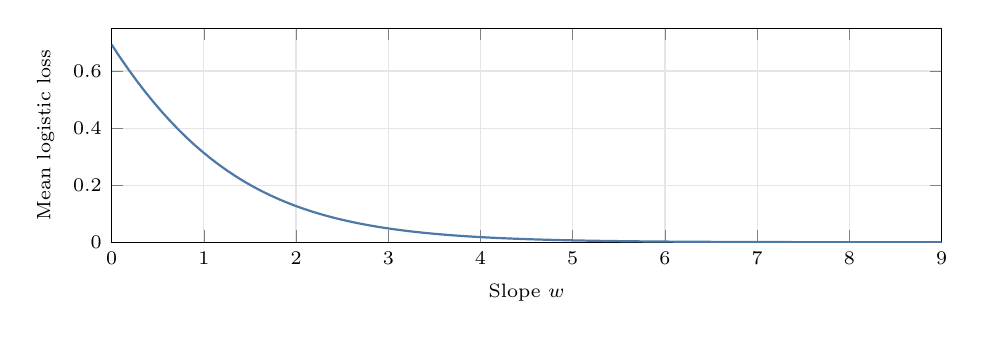
\begin{tikzpicture}\begin{axis}[width=\linewidth,height=4.3cm,xmin=0,xmax=9,ymin=0,ymax=.75,grid=major,grid style={black!10},xlabel={Slope $w$},ylabel={Mean logistic loss},font=\scriptsize,tick label style={font=\scriptsize},label style={font=\scriptsize}]
\addplot[blueplot,thick,domain=0:9,samples=101]{ln(1+exp(-x))};
\end{axis}\end{tikzpicture}
\end{column}
\begin{column}{.41\textwidth}\small
Two observations: $(-1,0)$ and $(1,1)$; let $b=0$.
\[
J(w)=\log(1+e^{-w}).
\]
\[
J(w)\downarrow0\quad\text{as }w\to\infty.
\]
No finite $w$ attains zero loss.
\end{column}
\end{columns}
\begin{takeaway}A vanishing loss can accompany exploding coefficients. Regularization can prevent this behavior.\end{takeaway}
\note{This simple full-rank two-observation example is completely separable. The infimum is zero but no finite unregularized maximum-likelihood estimate exists. For this example adding lambda w squared over two with lambda>0 yields a finite optimum. In general an unpenalized intercept can still diverge when only one class is observed. Near separation also leads to weak curvature.}
\end{frame}

% Plan: numerical implementation / equivalent loss formula / static.
\begin{frame}[t]{Evaluate the loss without overflow}
\begin{definitionbox}
\[
\ell(y,z)=\log(1+e^z)-yz
=\boxed{\max(z,0)-yz+\log(1+e^{-|z|})}.
\]
\end{definitionbox}
\small
\begin{itemize}\setlength{\itemsep}{.24cm}
\item Compute cross-entropy directly from scores (logits).
\item Avoid taking $\log$ of probabilities rounded to $0$ or $1$.
\item Check training loss, held-out performance, and coefficient size.
\end{itemize}
\end{frame}

\SectionSlide{Multiclass Classification}{}
% Final main lecture section. Requires theme.tex and logistic-macros.tex.
% Notation: raw x_i has p-1 coordinates; augmented tilde x_i is a p-vector.
% Rows of X are the transposes of augmented tilde x_i, including the intercept.
% W is p x K, with one class parameter vector per column.
% All figures are original analytical teaching examples, not measured data.
\section{Softmax regression}

% S01 POINT: A categorical task needs one distribution over mutually exclusive labels.
% LAYOUT: Short motivation above a three-row table. REVEAL: Static.
\begin{frame}{One item, one defect label}
  \lead{An inspection system records the primary defect on each rejected item.}
  \begin{center}
    \renewcommand{\arraystretch}{1.3}
    \begin{tabular}{cll}
      \toprule
      Class & Label & Possible visual evidence \\
      \midrule
      \textcolor{blueplot}{$1$} & Scratch & Elongated surface mark \\
      \textcolor{redplot}{$2$} & Dent & Local indentation \\
      $3$ & Stain & Discolored region \\
      \bottomrule
    \end{tabular}
  \end{center}
  \begin{definitionbox}
    The model assigns $\pi_k(x)=\Pr(y=k\mid x)$ for $k=1,2,3$,
    with $\pi_1(x)+\pi_2(x)+\pi_3(x)=1$.
  \end{definitionbox}
  \note{This is a constructed inspection task, not an empirical dataset. The label policy selects one primary defect even if several physical defects could coexist. If the task instead records every defect present, it becomes a multilabel problem and the categorical model here no longer expresses that target. Ask students what information is lost by collapsing all three labels into defective versus nondefective. Reference for the categorical setup: CS229 notes, Section 2.3, \url{https://cs229.stanford.edu/main_notes.pdf}.}
\end{frame}

% S02 POINT: Each class has a linear score, with classes stored as columns.
% LAYOUT: Definition box and dimension equation. REVEAL: Static.
\begin{frame}{One linear score for each class}
  \lead{For $x\in\R^{p-1}$, include the intercept in $\widetilde x=(1,x^\top)^\top\in\R^p$.}
  \begin{definitionbox}
    \[
      z_k(x)=\widetilde x^\top w_k,\qquad
      W=[\,w_1\ \cdots\ w_K\,]\in\R^{p\times K}.
    \]
    The real-valued scores $z_k$ are called \textbf{logits}.
  \end{definitionbox}
  \[
    \underbrace{Z}_{n\times K}
    =\underbrace{X}_{n\times p}\,
     \underbrace{W}_{p\times K}.
  \]
  \begin{itemize}
    \item Row $i$ of $X$ is $\widetilde x_i^\top$.
    \item Each column of $W$ describes one class.
  \end{itemize}
  \note{The raw feature vector is x. Its augmented vector is tilde x, with a leading one. Each row of X is the transpose of an augmented vector, so the first column of X consists of ones and the first row of W holds the K intercepts. This orientation matters later: X transposed times a matrix of probability residuals has exactly the same p by K shape as W. A logit is an unrestricted real score. It becomes a log odds only after taking a difference between two class scores. Source: CS229 notes, Section 2.3, \url{https://cs229.stanford.edu/main_notes.pdf}.}
\end{frame}

% S03 POINT: Exponentiation and shared normalization produce one categorical distribution.
% LAYOUT: Central definition and two consequences. REVEAL: Static.
\begin{frame}{Softmax probabilities}
  \begin{definitionbox}
    \[
      \pi_k(x)=\frac{\exp(z_k(x))}{\sum_{j=1}^{K}\exp(z_j(x))},
      \qquad k=1,\ldots,K.
    \]
  \end{definitionbox}
  \begin{itemize}
    \item Finite logits give positive probabilities that sum to one.
    \item Every class shares the same denominator.
  \end{itemize}
  \[
    \widehat y(x)=\operatorname*{arg\,max}_{k}\pi_k(x)
                 =\operatorname*{arg\,max}_{k}z_k(x).
  \]
  \begin{takeaway}
    Predicting a label requires only the largest score.
    Likelihood training uses the entire normalized distribution.
  \end{takeaway}
  \note{Exponentiation preserves score ordering, and the common positive denominator preserves it again. The displayed decision rule minimizes expected zero-one loss under the model, with a fixed rule for ties. Different error costs can require a different decision rule. Contrast the shared denominator with independently fitted binary probabilities: K independent sigmoid outputs need not sum to one. Source: CS229 notes, Section 2.3, \url{https://cs229.stanford.edu/main_notes.pdf}.}
\end{frame}

% S04 POINT: Score differences, not raw magnitudes, determine a concrete probability vector.
% LAYOUT: Numerical table left, native probability bars right.
% REVEAL: Scores/exponentials first; probabilities and bars on step 2 (uncover).
\begin{frame}{Three scores, three probabilities}
  \lead{Constructed example: $z=(2,1,0)^\top$.}
  \begin{columns}[T,onlytextwidth]
    \begin{column}{0.47\textwidth}
      \vspace{0.15cm}
      \small
      \renewcommand{\arraystretch}{1.35}
      \begin{tabular}{lrrr}
        \toprule
        Class & $z_k$ & $e^{z_k}$ & $\pi_k$ \\
        \midrule
        Scratch & $2$ & $7.389$ & \uncover<2->{$0.665$} \\
        Dent & $1$ & $2.718$ & \uncover<2->{$0.245$} \\
        Stain & $0$ & $1.000$ & \uncover<2->{$0.090$} \\
        \bottomrule
      \end{tabular}
      \vspace{0.25cm}
      \par The normalizer is $11.107$.
      \uncover<2->{\par A one-unit score advantage multiplies the probability ratio by $e$.}
    \end{column}
    \begin{column}{0.50\textwidth}
      \uncover<2->{\logfig{softmax-probabilities}}
    \end{column}
  \end{columns}
  \note{These values come directly from the analytical softmax formula and are rounded only for display. The exact probabilities are approximately 0.665240956, 0.244728471, and 0.090030573. Scratch is the predicted class, but the other classes retain positive probability. A ratio such as pi1 divided by pi2 equals exp(2 minus 1), without needing the normalizing constant. The example is original. Formula reference: \url{https://cs229.stanford.edu/main_notes.pdf}, Section 2.3.}
\end{frame}

% S05 POINT: Conditional categorical likelihood turns observed labels into a fitting criterion.
% LAYOUT: One-hot definition, likelihood, MLE.
% REVEAL: Categorical likelihood first; MLE and interpretation on step 2 (uncover).
\begin{frame}{Categorical likelihood}
  \lead{Write $Y_{ik}=\mathbf{1}\{y_i=k\}$ and $P_{ik}=\pi_k(x_i)$.}
  \[
    L(W)=\prod_{i=1}^{n}\prod_{k=1}^{K}P_{ik}^{Y_{ik}}
        =\prod_{i=1}^{n}P_{i,y_i}.
  \]
  \uncover<2->{\begin{definitionbox}
    \[
      \widehat W\in\operatorname*{arg\,max}_{W}\log L(W)
      =\operatorname*{arg\,max}_{W}
        \sum_{i=1}^{n}\sum_{k=1}^{K}Y_{ik}\log P_{ik}.
    \]
  \end{definitionbox}
  \begin{itemize}
    \item The observed class selects one probability from each row.
    \item The product assumes conditionally independent labels given the inputs.
  \end{itemize}}
  \note{Condition on the observed design X. The one-hot vector contains exactly one entry equal to one, so each categorical likelihood term reduces to the probability assigned to the observed class. The argmax notation describes the maximum-likelihood objective. A finite maximizer can fail to exist on separable data, as in binary logistic regression, and the unrestricted K-column parameterization has a common-shift ambiguity discussed shortly. No optimization algorithm is introduced here. Source: CS229 notes, Section 2.3, \url{https://cs229.stanford.edu/main_notes.pdf}.}
\end{frame}

% S06 POINT: Cross-entropy is the average negative log-likelihood and has a simple logit form.
% LAYOUT: Two displayed equations and one numerical interpretation.
% REVEAL: Average cross-entropy first; logit form and example on step 2 (uncover).
\begin{frame}{Cross-entropy and log-sum-exp}
  \[
    J(W)=-\frac{1}{n}\log L(W)
    =-\frac{1}{n}\sum_{i=1}^{n}\sum_{k=1}^{K}Y_{ik}\log P_{ik}.
  \]
  \uncover<2->{\begin{definitionbox}
    For one observation with true class $y$,
    \[
      \ell(z,y)
      =\underbrace{\log\!\left(\sum_{k=1}^{K}e^{z_k}\right)}_{
        \operatorname{LSE}(z)}-z_y.
    \]
  \end{definitionbox}
  \begin{takeaway}
    For $z=(2,1,0)^\top$ and true class Dent,
    the loss is $-\log(0.2447)\approx1.408$ nats.
  \end{takeaway}}
  \note{Substitute log P_ik equals z_ik minus log-sum-exp of the row. Since the one-hot row sums to one, the normalization term appears once, leaving LSE(z) minus the true class score. Natural logarithms measure the loss in nats. For the same logits, the losses for Scratch, Dent, and Stain are about 0.407606, 1.407606, and 2.407606. The example illustrates that the probability of the observed label controls the loss even when the predicted label stays unchanged. Source: CS229 notes, Section 2.3, \url{https://cs229.stanford.edu/main_notes.pdf}.}
\end{frame}

% S07 POINT: The categorical gradient is the matrix form of probability minus target.
% LAYOUT: Per-logit derivative above dimensioned matrix gradient. REVEAL: Static.
\begin{frame}{The gradient is a probability residual}
  \[
    \frac{\partial\ell(z_i,y_i)}{\partial z_{ik}}
       =P_{ik}-Y_{ik}.
  \]
  \begin{definitionbox}
    \[
      \underbrace{\nabla_W J}_{p\times K}
        =\frac{1}{n}\,
          \underbrace{X^\top}_{p\times n}
          \underbrace{(P-Y)}_{n\times K}.
    \]
  \end{definitionbox}
  \begin{itemize}
    \item $P$ applies softmax independently to each row of $XW$.
    \item Each class column accumulates feature-weighted probability errors.
  \end{itemize}
  \note{Differentiate log-sum-exp to obtain softmax, then differentiate minus the selected score to obtain minus the one-hot target. Apply the chain rule to z_ik equals augmented tilde x_i transposed w_k and average across observations. The design X has those augmented feature vectors as rows. This gives the displayed p by K matrix without a transposition ambiguity. Because each row of P minus Y sums to zero, the gradient columns also sum to zero. That identity foreshadows the common-shift invariance. The formula is for the unregularized mean negative log-likelihood. Source: CS229 notes, equations 2.16--2.19, \url{https://cs229.stanford.edu/main_notes.pdf}.}
\end{frame}

% S08 POINT: Binary logistic regression uses the difference of two softmax logits.
% LAYOUT: Binary identity followed by general pairwise log odds. REVEAL: Static.
\begin{frame}{Binary logistic regression is the $K=2$ case}
  \[
    \pi_1(x)
      =\frac{e^{z_1}}{e^{z_1}+e^{z_2}}
      =\frac{1}{1+e^{-(z_1-z_2)}}
      =\sigm\!\left(\widetilde x^\top(w_1-w_2)\right).
  \]
  \begin{definitionbox}
    For any pair of classes,
    \[
      \log\frac{\pi_j(x)}{\pi_k(x)}
        =z_j(x)-z_k(x)=\widetilde x^\top(w_j-w_k).
    \]
  \end{definitionbox}
  \begin{takeaway}
    Softmax regression makes every pairwise log odds linear in the features.
  \end{takeaway}
  \note{For the binary comparison, map class 1 to binary target one and class 2 to binary target zero. The binary coefficient vector is the difference w1 minus w2. Setting w2 to zero recovers the familiar single-vector logistic parameterization. For K classes, a single logit has no absolute probabilistic meaning. Its difference from another logit specifies their log probability ratio. These identities are algebraic consequences of softmax. Background definitions: \url{https://cs229.stanford.edu/main_notes.pdf}, Sections 2.1 and 2.3.}
\end{frame}

% S09 POINT: Common score shifts produce identical distributions, so choose a reference.
% LAYOUT: Invariance equation and baseline parameterization. REVEAL: Static.
\begin{frame}{A reference class removes redundant parameters}
  \[
    \operatorname{softmax}(z+c\mathbf{1})
      =\operatorname{softmax}(z),\qquad c\in\R.
  \]
  \lead{Adding the same $a\in\R^p$ to every column of $W$ changes no prediction.}
  \begin{definitionbox}
    Choose class $K$ as the baseline:
    \[
      w'_k=w_k-w_K\ (k<K),\qquad w'_K=0.
    \]
    This leaves $(K-1)p$ free coefficients.
  \end{definitionbox}
  \begin{itemize}
    \item The fitted probabilities survive the change of coordinates.
    \item The baseline fixes this ambiguity, not rank deficiency or separation.
  \end{itemize}
  \note{The common factor exp(c) cancels in numerator and denominator. At parameter level, replacing W by W plus a times the all-ones row adds c(x)=tilde x transposed a to every score for that input. Here tilde x is the augmented feature vector. Subtracting w_K from all columns therefore preserves the entire conditional distribution. A sum-to-zero constraint is another possible convention. Additional data conditions are needed for a unique finite maximum-likelihood solution. A penalty can select a representative, so a penalty specified in one parameterization must be transformed carefully before claiming equivalence to another. The proof here is direct algebra from the softmax definition in \url{https://cs229.stanford.edu/main_notes.pdf}.}
\end{frame}

% S10 POINT: Subtracting the row maximum avoids exponent overflow without changing probabilities.
% LAYOUT: Stable probability and loss equations. REVEAL: Static.
\begin{frame}{Stable computation uses score differences}
  \lead{For one row, set $m=\max_k z_k$.}
  \[
    \pi_k=\frac{e^{z_k-m}}{\sum_j e^{z_j-m}}.
  \]
  \begin{definitionbox}
    \[
      \ell(z,y)=(m-z_y)+\log\sum_j e^{z_j-m}.
    \]
    Every exponential is at most $1$, and at least one equals $1$.
  \end{definitionbox}
  \begin{takeaway}
    $(1002,1001,1000)$ gives exactly the same probabilities as $(2,1,0)$.
    Compute the loss from logits to avoid taking $\log(0)$ after underflow.
  \end{takeaway}
  \note{This is a numerical use of common-shift invariance, distinct from choosing a fixed baseline class to parameterize the model. Large negative shifted logits can underflow to zero, but the denominator still contains a one. Computing the log-likelihood directly in the displayed form retains a finite loss for ordinary finite logits even when a tiny probability would round to zero. Prefer a library's fused log-softmax or cross-entropy operation. The subtract-maximum procedure is described in Bengio et al., A Neural Probabilistic Language Model, page 1146, \url{https://www.jmlr.org/papers/volume3/bengio03a/bengio03a.pdf}.}
\end{frame}

% S11 POINT: Linear logits create linear winning-class boundaries in the feature plane.
% LAYOUT: Two-dimensional native decision-region figure with compact equations. REVEAL: Static.
\begin{frame}{Three classes partition the feature plane}
  \begin{columns}[T,onlytextwidth]
    \begin{column}{0.58\textwidth}
      \logfig{softmax-boundaries}
    \end{column}
    \begin{column}{0.39\textwidth}
      \small
      Constructed scores:
      \[
        z_1=u_1,\quad z_2=u_2,\quad z_3=0.
      \]
      A boundary between winning classes $j$ and $k$ satisfies
      \[
        \widetilde x^\top(w_j-w_k)=0.
      \]
      Here $\widetilde x=(1,u_1,u_2)^\top$.
      \par Black segments mark ties for the largest score.
    \end{column}
  \end{columns}
  \note{The regions are analytical, not estimated from a dataset. Class 1 wins when u1 is at least u2 and at least zero. Class 2 wins when u2 is at least u1 and at least zero. Class 3 wins when both features are nonpositive. A pairwise equality line is an actual decision boundary only where those tied classes achieve the largest score. For example, the negative part of u1 equals u2 lies inside class 3 and is not a boundary. The geometry is linear in the chosen features. A nonlinear learned feature map can yield curved boundaries in the original inputs. Reference for the underlying logits: \url{https://cs229.stanford.edu/main_notes.pdf}.}
\end{frame}

% S12 POINT: Temperature changes confidence for fixed logits without changing their order.
% LAYOUT: Analytical temperature curves and two caveats. REVEAL: Static.
\begin{frame}{Temperature changes concentration}
  \begin{columns}[T,onlytextwidth]
    \begin{column}{0.55\textwidth}
      \logfig{softmax-temperature}
    \end{column}
    \begin{column}{0.42\textwidth}
      \small
      For fixed logits and $T>0$,
      \[
        \pi_k(T)=\frac{e^{z_k/T}}{\sum_j e^{z_j/T}}.
      \]
      \begin{itemize}
        \item Larger $T$ spreads probability more evenly.
        \item The largest score and predicted class stay unchanged.
      \end{itemize}
    \end{column}
  \end{columns}
  \begin{takeaway}
    Softer probabilities do not automatically imply better calibration.
    Fit a calibration temperature on held-out labeled data.
  \end{takeaway}
  \note{The graph fixes z=(2,1,0). As T tends to infinity the distribution approaches uniform. As T tends to zero from above it concentrates on the unique maximum here; tied maxima would share the limiting mass. Positive temperature preserves all score orderings, although it changes sampling behavior. Calibration concerns whether predicted probabilities match observed frequencies over data, not how uncertain one output looks. A temperature chosen to minimize held-out negative log-likelihood is a fitted calibration method, with generalization assessed separately. Source: Guo et al., On Calibration of Modern Neural Networks, Section 4, \url{https://proceedings.mlr.press/v70/guo17a/guo17a.pdf}.}
\end{frame}

% S13 POINT: Learned features let the same categorical output likelihood serve vision and language.
% LAYOUT: Two vertically separated application equations. REVEAL: Static.
\begin{frame}{Categorical outputs in vision and language}
  \textbf{Image classification}\par\vspace{-2pt}
  \[
    \Pr(y=k\mid\text{image})
      =\operatorname{softmax}\!\left(A^\top h(\text{image})+b\right)_k.
  \]
  {\small AlexNet used a 1000-class softmax output above learned visual features.}

  \vspace{0.18cm}
  \textbf{Next-token prediction}\par\vspace{-2pt}
  \[
    \Pr(v_t=k\mid v_{<t})=\operatorname{softmax}(z_t)_k,
    \qquad J_{\mathrm{seq}}=-\sum_t\log\Pr(v_t\mid v_{<t}).
  \]
  {\small The observed next token selects one vocabulary probability at each position.}
  \note{A neural classifier can learn h jointly with its linear output layer. Its final softmax has the categorical likelihood studied here, while the full model can be nonlinear in the original input. AlexNet's 1000-way output and multinomial logistic objective are described in Section 3.5: \url{https://proceedings.neurips.cc/paper_files/paper/2012/file/c399862d3b9d6b76c8436e924a68c45b-Paper.pdf}. Neural language models also use a categorical output distribution, historically over words and now often over subword tokens. Bengio et al. give the softmax output and corpus log-likelihood on page 1142: \url{https://www.jmlr.org/papers/volume3/bengio03a/bengio03a.pdf}. The Transformer's decoder-output softmax appears in Section 3.4: \url{https://arxiv.org/html/1706.03762v7}. The sequence factorization conditions on preceding tokens; it does not assume the tokens themselves are independent.}
\end{frame}

% S14 POINT: Attention normalizes weights over positions, which is a different statistical role.
% LAYOUT: Attention equation followed by a two-row comparison. REVEAL: Static.
\begin{frame}{Softmax also supplies attention weights}
  \[
    A=\operatorname{softmax}_{\mathrm{row}}\!\left(
      \frac{QK_{\!\mathrm{key}}^\top}{\sqrt{d_k}}\right),
    \qquad H=A V.
  \]
  \begin{center}
    \small
    \renewcommand{\arraystretch}{1.4}
    \begin{tabularx}{0.97\textwidth}{lYY}
      \toprule
      Use & Normalize over & Meaning of an entry \\
      \midrule
      Output classifier & Classes or vocabulary & Probability of a target label \\
      Attention row & Available key positions & Weight in a mixture of value vectors \\
      \bottomrule
    \end{tabularx}
  \end{center}
  \begin{takeaway}
    Softmax attention is not itself a label-likelihood classifier.
    Its weights help construct the representations used for prediction.
  \end{takeaway}
  \note{For each query, softmax normalizes compatibility scores across available key positions. The resulting row weights mix value vectors. In the displayed equation, K_key denotes the key matrix, distinct from the number K of output classes, and d_k is the key dimension. Without dropout, and with at least one allowed key, each attention row sums to one. Causal masks remove forbidden positions before normalization. The standard attention layer does not assign a categorical target label to each query and train that row with the supervised label likelihood derived earlier. The output layer can separately use a softmax over vocabulary with a token likelihood. Source: Vaswani et al., Attention Is All You Need, Sections 3.2.1 and 3.4, \url{https://arxiv.org/html/1706.03762v7}; canonical paper record: \url{https://arxiv.org/abs/1706.03762}.}
\end{frame}

% Plan: synthesis / response-family comparison / static.

% Plan: readable references / annotated list / static.
\begin{frame}[t]{References and further reading}
\small
\begin{itemize}\setlength{\itemsep}{.20cm}
\item Ma and Ng. \href{https://cs229.stanford.edu/main_notes.pdf}{\textit{CS229 Lecture Notes}.}\par
Gaussian least squares, logistic regression, and softmax.
\item Krizhevsky, Sutskever, and Hinton (2012).\par
\href{https://proceedings.neurips.cc/paper_files/paper/2012/file/c399862d3b9d6b76c8436e924a68c45b-Paper.pdf}{\textit{ImageNet Classification with Deep Convolutional Neural Networks}.}
\item Bengio et al. (2003).\par
\href{https://www.jmlr.org/papers/volume3/bengio03a/bengio03a.pdf}{\textit{A Neural Probabilistic Language Model}.}
\item Vaswani et al. (2017). \href{https://arxiv.org/abs/1706.03762}{\textit{Attention Is All You Need}.}
\item Guo et al. (2017). \href{https://proceedings.mlr.press/v70/guo17a.html}{\textit{On Calibration of Modern Neural Networks}.}
\end{itemize}
\note{All titles are clickable in the PDF. The source package records the exact primary-source URLs and sections used. Every plotted observation, curve, and worked number in this lecture is either an explicit analytical construction or a reproducible computation on constructed teaching data. No figure is presented as a measured industrial performance result. The Gaussian/logistic derivations also follow the earlier 2022 CS229 notes, \url{https://cs229.stanford.edu/notes2022fall/main_notes.pdf}.}
\end{frame}

\end{document}
